% ------------------------------------------------------------
\chapter{IMPLEMENTATION}
\setlength{\parindent}{0pt}
\setlength{\parskip}{6pt}
{\setstretch{1.5}

This chapter describes the practical implementation of the ResQNow emergency response system through detailed pseudocode and code snippets.  It explains how the core functionalities—SOS alert triggering, Bluetooth Low Energy (BLE) based offline communication, and AI-driven emergency classification—were developed and integrated. 

% -----------------------------------------------------------------------------
\section{SOS Activation and Emergency Alert Implementation}

The SOS module serves as the primary emergency trigger in ResQNow. Upon activation, the system captures GPS location, timestamps the event, and initiates alert propagation through available communication channels. 

\subsection{SOS Activation Pseudocode}

Algorithm~\ref{alg:sos_activation} demonstrates the entire lifecycle of SOS initiation, detailing how the application processes an emergency request from the moment the user triggers it. The workflow begins when an SOS input is received via a button press or voice command, after which the system immediately retrieves the user’s real-time GPS coordinates and authenticated user identity. These details are encapsulated into a structured SOS data object, which also includes a timestamp and initializes severity status as pending. The algorithm further incorporates an intelligent connectivity check—if the device has internet access, the alert is transmitted to the backend server and emergency contacts receive notifications instantly. In case of offline conditions, the message is queued locally and broadcasted using BLE so nearby devices can relay it until it reaches a device with network access, ensuring message delivery even in network-restricted environments. This design guarantees resilience and reliability in emergency situations.

\begin{algorithm}[H]
\caption{SOS Activation and Alert Dispatch}
\label{alg:sos_activation}
\begin{algorithmic}[1]
\State \textbf{Input:} User trigger (button press or voice command)
\State \textbf{Output:} SOS alert dispatched to backend and emergency contacts
\State
\Procedure{ActivateSOS}{}
    \State $location \gets$ \Call{GetGPSLocation}{}
    \State $timestamp \gets$ \Call{GetCurrentTimestamp}{}
    \State $userId \gets$ \Call{GetAuthenticatedUserId}{}
    \State
    \State $sosData \gets$ \{
    \State \hspace{1cm} userId: $userId$,
    \State \hspace{1cm} latitude: $location.latitude$,
    \State \hspace{1cm} longitude:  $location.longitude$,
    \State \hspace{1cm} timestamp: $timestamp$,
    \State \hspace{1cm} severity: "pending\_classification"
    \State \}
    \State
    \If{InternetAvailable()}
        \State \Call{SendSOSToBackend}{$sosData$}
        \State \Call{NotifyEmergencyContacts}{$sosData$}
    \Else
        \State \Call{QueueForBLERelay}{$sosData$}
        \State \Call{InitiateBLEBroadcast}{$sosData$}
    \EndIf
    \State
    \State \Call{DisplayConfirmation}{"SOS Alert Activated"}
\EndProcedure
\end{algorithmic}
\end{algorithm}

\subsection{SOS Implementation Code}

Figure~\ref{fig:sos_code} presents the Dart implementation of the SOS activation module, highlighting how the system programmatically handles emergency initiation. The \texttt{activateSOS()} function first utilizes the Geolocator package to fetch the device's GPS coordinates with high accuracy, applying a timeout of 10 seconds to prevent indefinite waits. Once the location is retrieved, the function obtains the authenticated user’s UID from Firebase Authentication and constructs an SOS payload that encapsulates latitude, longitude, timestamp formatted in ISO 8601, and a default severity status. To determine the appropriate dispatch path, the function performs a network availability check using the Connectivity package. If internet connectivity is available, the SOS payload is transmitted to the backend server via HTTP POST request and emergency contacts are notified immediately. In offline conditions, the alert is stored in a local SQLite queue for persistence and a BLE broadcast is initiated to enable peer-to-peer relay until a device with connectivity is reached.
\begin{figure}[H]
    \centering
    \includegraphics[width=0.95\textwidth]{chapters/sos_code.png}
    \caption{SOS activation implementation showing location capture, connectivity check, and alert dispatch logic}
    \label{fig:sos_code}
\end{figure}

% -----------------------------------------------------------------------------
\section{Bluetooth Low Energy (BLE) Offline Communication Implementation}

To support emergency alert delivery in low or no internet connectivity environments, ResQNow implements BLE-based offline SOS relay.  The BLE module discovers nearby devices and establishes secure short-range connections for message forwarding. 

\subsection{BLE Message Relay Pseudocode}

Algorithm~\ref{alg:ble_relay} presents the BLE relay process used when internet connectivity is unavailable. The originating device encrypts the SOS data using AES-128 and scans for nearby ResQNow devices. If available, the encrypted message is transmitted via GATT; otherwise, it is queued and retried after a delay. Receiving devices decrypt the payload and either upload it to the server if online or forward it to other devices, forming a lightweight mesh network for offline alert propagation.

\begin{algorithm}[H]
\caption{BLE Offline SOS Relay}
\label{alg:ble_relay}
\begin{algorithmic}[1]
\State \textbf{Input:} SOS message
\State \textbf{Output:} Delivered to an internet-active device
\Procedure{InitiateBLERelay}{$msg$}
\State $enc \gets$ EncryptAES($msg$)
\State $devices \gets$ ScanForBLEDevices()
\If{$devices \neq \emptyset$}
\For{$d$ in $devices$}
\State Connect($d$); Send($d$, $enc$)
\EndFor
\Else
\State Queue($enc$); Retry(5s)
\EndIf
\EndProcedure
\Procedure{ReceiveBLE}{$encMsg$, $src$}
\State $msg \gets$ DecryptAES($encMsg$)
\If{InternetAvailable()} \State Upload($msg$); Ack($src$)
\Else \State Relay($encMsg$)
\EndIf
\EndProcedure
\end{algorithmic}
\end{algorithm}

\subsection{BLE Implementation Code}

The following code snippet implements BLE communication using the flutter\_blue\_plus package.  The \texttt{initiateBLERelay()} function begins by converting the SOS data to JSON and encrypting it using the encrypt package with AES-128 in GCM mode, generating a random initialization vector for each message. The \texttt{scanForDevices()} method initiates a 10-second BLE scan filtered by the ResQNow service UUID (defined as a constant). For each discovered device, the code establishes a connection, discovers services, locates the SOS relay characteristic, and writes the encrypted payload.  The \texttt{onMessageReceived()} callback handles incoming messages by decrypting the payload, parsing the JSON, checking connectivity, and either uploading to Firebase or calling \texttt{relayToOthers()} to continue the mesh relay. Error handling includes connection timeouts, encryption failures, and retry logic. Figure~\ref{fig:ble_code} presents this implementation.

\begin{figure}[H]
    \centering
    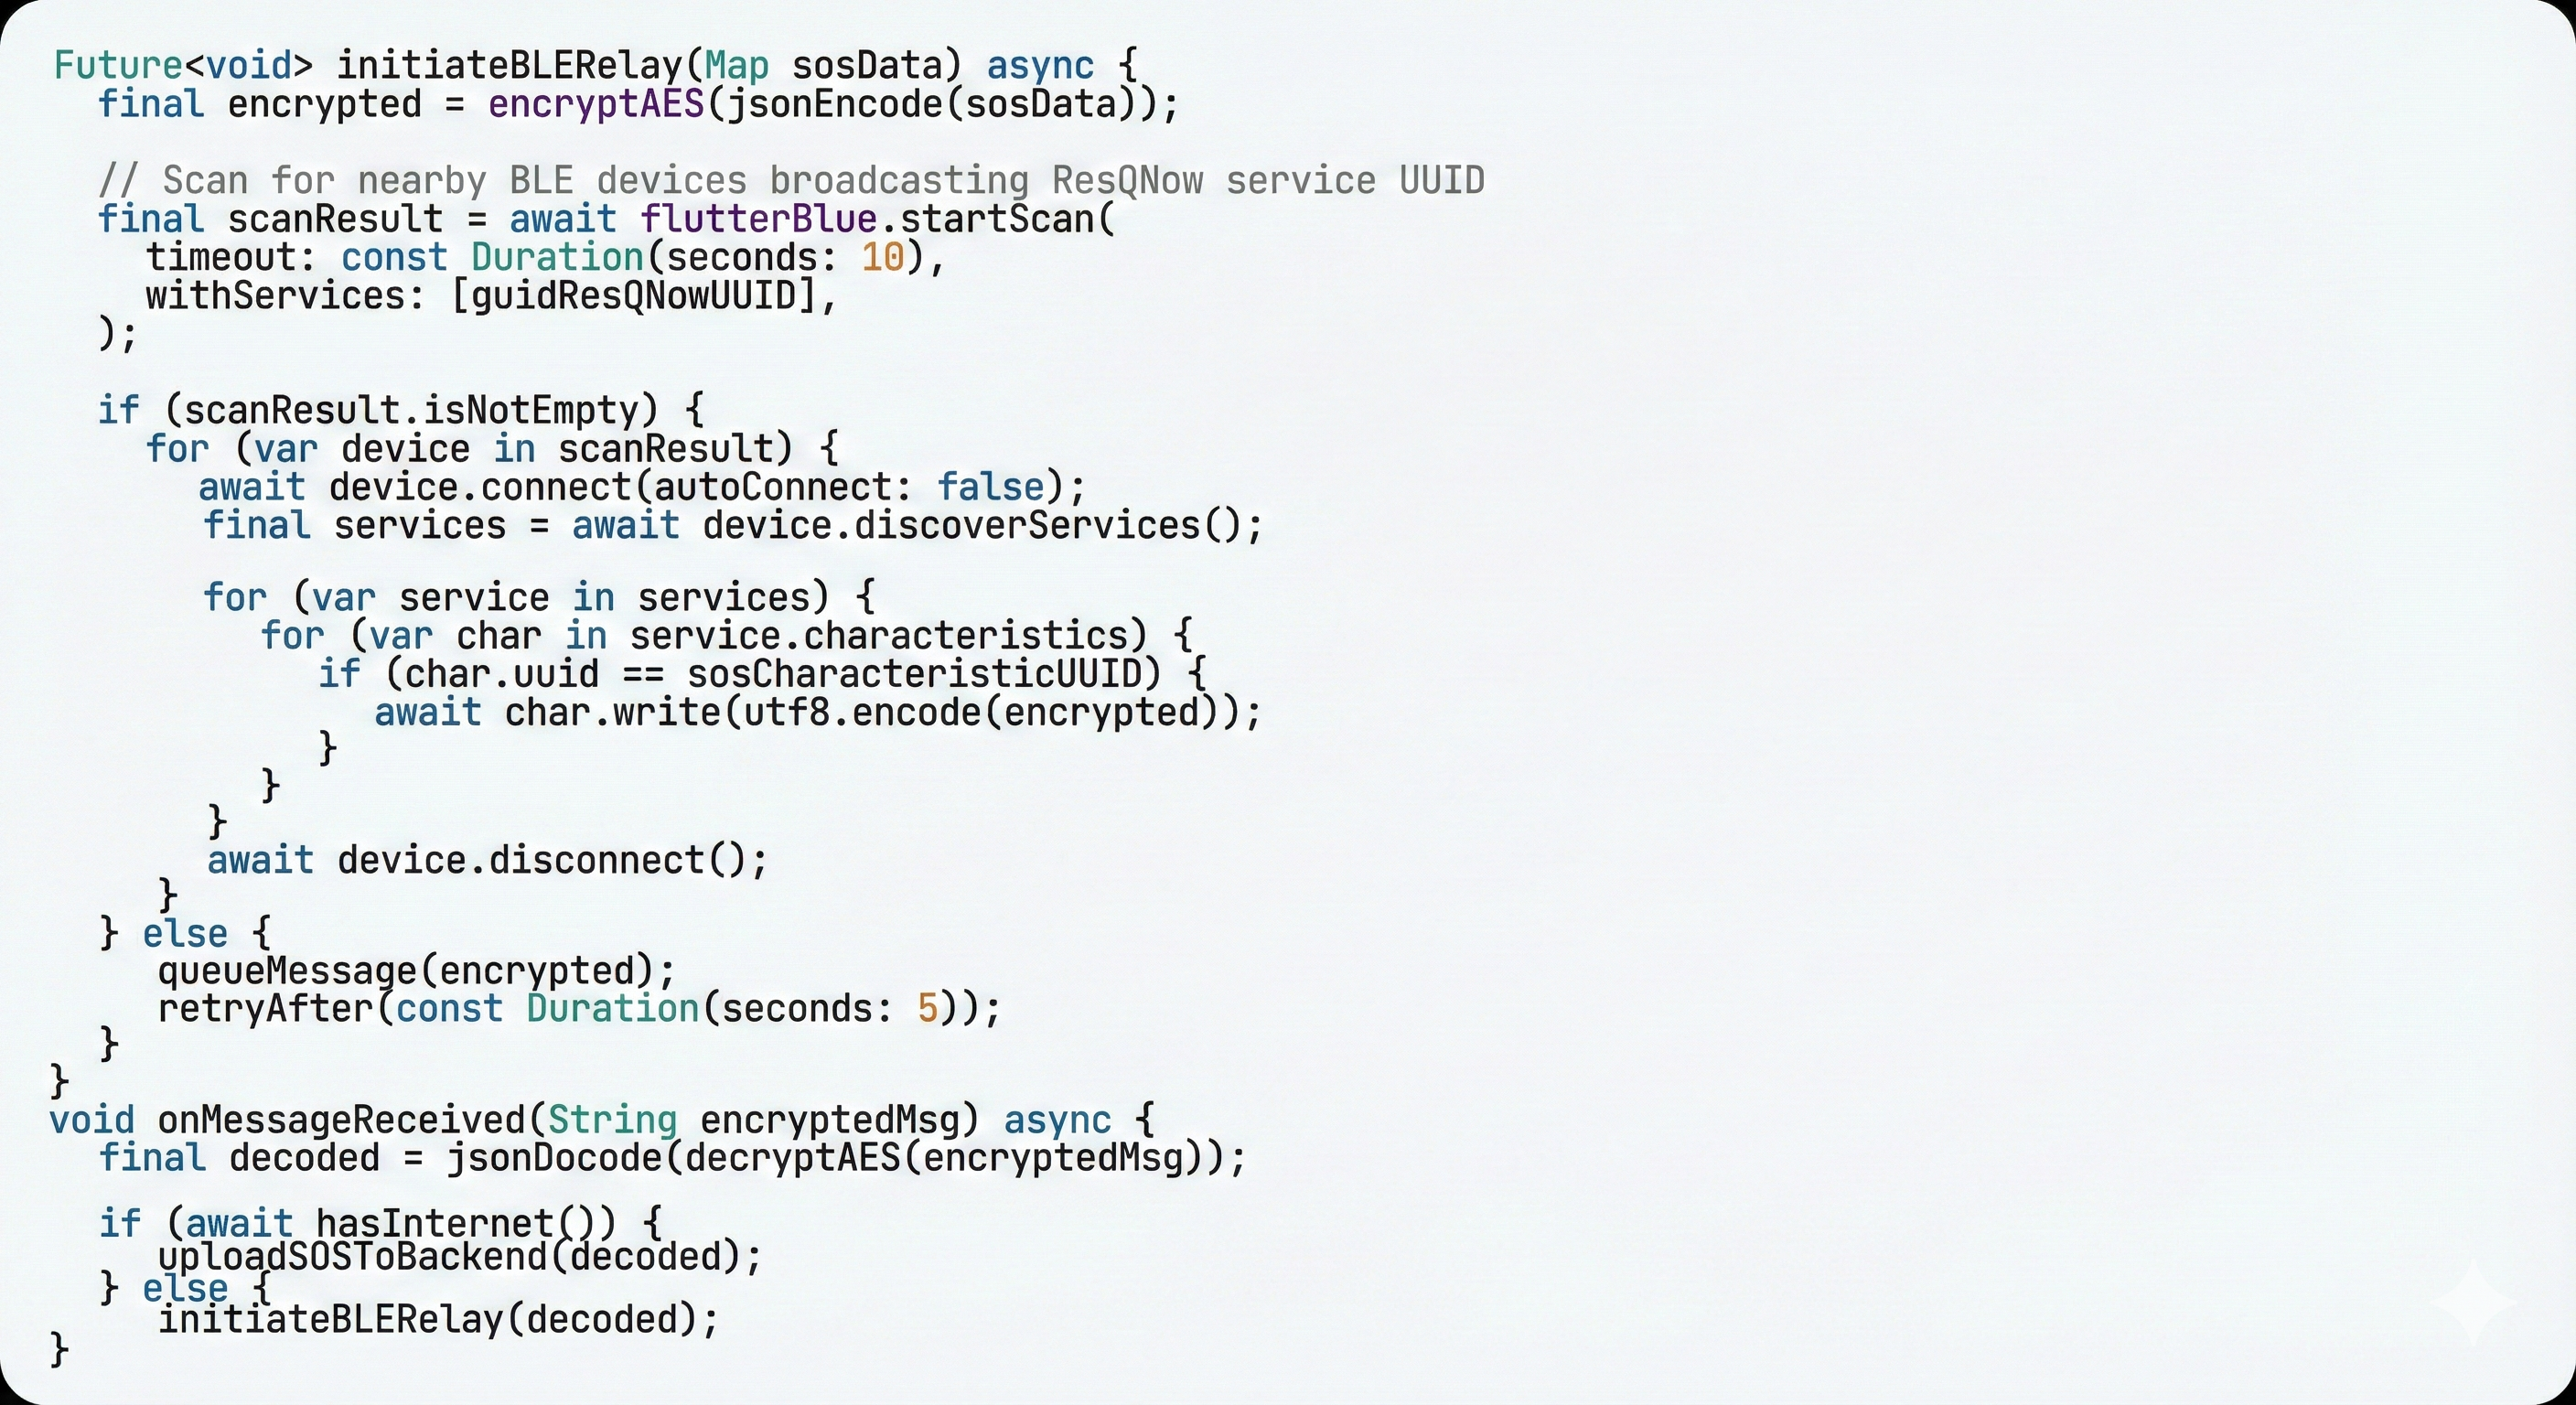
\includegraphics[width=0.95\textwidth]{chapters/ble_code.png}
    \caption{BLE relay implementation with AES encryption, device scanning, and mesh relay logic}
    \label{fig:ble_code}
\end{figure}

% -----------------------------------------------------------------------------
\section{AI-Based Emergency Classification Implementation}

Artificial Intelligence enables ResQNow to automatically analyze user inputs and prioritize emergency handling based on severity and type. The system employs a hybrid approach combining cloud-based AI for detailed analysis and rule-based logic for offline scenarios.

\subsection{AI Classification Pseudocode}

The AI classification process begins by checking network availability to determine which classification method to use. When online, the system sends the user's emergency description to a cloud AI service (Google Gemini or OpenAI GPT) via API call. The response is parsed to extract the predicted emergency type (cardiac arrest, severe bleeding, burn injury, fracture, or general emergency) and severity level (HIGH, MODERATE, or LOW). If the AI returns a confidence score below 0.7, indicating uncertainty, the system supplements or overrides the result using rule-based fallback logic. When offline, the system relies entirely on rule-based classification, which extracts keywords from the user input and matches them against predefined patterns. Keywords like "unconscious" or "not breathing" trigger HIGH severity cardiac arrest classification, while "bleeding" triggers severe bleeding, and so on. Algorithm~\ref{alg: ai_classification} outlines this process. 

\begin{algorithm}[H]
\caption{AI-Based Emergency Classification}
\label{alg: ai_classification}
\begin{algorithmic}[1]
\State \textbf{Input:} User description of emergency (text or voice)
\State \textbf{Output:} Emergency type and severity level
\State
\Procedure{ClassifyEmergency}{$userInput$}
    \If{InternetAvailable()}
        \State $aiResponse \gets$ \Call{CloudAIClassification}{$userInput$}
        \State $emergencyType \gets$ \Call{ExtractType}{$aiResponse$}
        \State $severity \gets$ \Call{ExtractSeverity}{$aiResponse$}
        \State
        \If{$aiResponse.confidence < 0.7$}
            \State $severity \gets$ \Call{RuleBasedFallback}{$userInput$}
        \EndIf
    \Else
        \State $emergencyType \gets$ \Call{RuleBasedClassification}{$userInput$}
        \State $severity \gets$ \Call{RuleBasedSeverity}{$userInput$}
    \EndIf
    \State
    \State \Return \{type: $emergencyType$, severity: $severity$\}
\EndProcedure
\State
\Procedure{RuleBasedClassification}{$userInput$}
    \State $keywords \gets$ \Call{ExtractKeywords}{$userInput$}
    \State
    \If{"unconscious" OR "not breathing" in $keywords$}
        \State \Return \{type: "cardiac\_arrest", severity: "HIGH"\}
    \ElsIf{"bleeding" OR "blood" in $keywords$}
        \State \Return \{type: "severe\_bleeding", severity: "HIGH"\}
    \ElsIf{"burn" in $keywords$}
        \State \Return \{type: "burn\_injury", severity: "MODERATE"\}
    \ElsIf{"fracture" OR "broken" in $keywords$}
        \State \Return \{type: "fracture", severity: "MODERATE"\}
    \Else
        \State \Return \{type: "general\_emergency", severity: "LOW"\}
    \EndIf
\EndProcedure
\end{algorithmic}
\end{algorithm}

\subsection{AI Chatbot Implementation Code}

The following code snippet implements the AI-powered emergency chatbot using Google Gemini API. The \texttt{AIChatService} class maintains conversation history as a list of message objects to enable multi-turn interactions. The \texttt{classifyEmergency()} function constructs a prompt that includes the system instruction (defining the AI's role as an emergency classifier), conversation history for context, and the current user message. It sends an HTTP POST request to the Gemini API endpoint with the API key and receives a JSON response containing the generated text, confidence score, and extracted emergency details. The \texttt{parseResponse()} method uses regular expressions to extract emergency type and severity from the AI's natural language response. The \texttt{ruleBasedFallback()} function implements keyword matching using a Map of emergency keywords to classification results, iterating through the user input to find matches. Error handling includes API timeout (30 seconds), rate limiting with exponential backoff, and automatic fallback to rule-based classification on any API failure. Figure~\ref{fig:ai_code} presents this implementation. 

\begin{figure}[H]
    \centering
    \includegraphics[width=0.95\textwidth]{chapters/ai_code.png}
    \caption{AI chatbot implementation with Gemini API integration, conversation management, and rule-based fallback}
    \label{fig:ai_code}
\end{figure}

% -----------------------------------------------------------------------------
\section{Emergency Contact Notification Implementation}

The notification system ensures reliable alert delivery to emergency contacts through multiple redundant channels. 

\subsection{Multi-Channel Notification Pseudocode}

The notification dispatch mechanism retrieves the list of emergency contacts associated with the user who triggered the SOS alert. It generates a Google Maps URL containing the emergency location coordinates for easy navigation.  A notification message is constructed containing the severity level and location link.  For each emergency contact, the system sends notifications through three channels: push notification via Firebase Cloud Messaging using the contact's device token, SMS via Twilio API using the contact's phone number, and email via SendGrid API using the contact's email address. This multi-channel approach maximizes the probability of successful alert delivery even if one channel fails. Algorithm~\ref{alg:notification} describes this mechanism.

\begin{algorithm}[H]
\caption{Multi-Channel Emergency Notification}
\label{alg:notification}
\begin{algorithmic}[1]
\State \textbf{Input:} SOS alert data, emergency contact list
\State \textbf{Output:} Notifications sent via multiple channels
\State
\Procedure{NotifyEmergencyContacts}{$sosData$}
    \State $contacts \gets$ \Call{GetEmergencyContacts}{$sosData. userId$}
    \State $locationURL \gets$ \Call{GenerateMapURL}{$sosData.latitude$, $sosData.longitude$}
    \State $message \gets$ "Emergency Alert: " + $sosData.severity$ + " at " + $locationURL$
    \State
    \For{each $contact$ in $contacts$}
        \State \Call{SendPushNotification}{$contact. deviceToken$, $message$}
        \State \Call{SendSMS}{$contact.phoneNumber$, $message$}
        \State \Call{SendEmail}{$contact. email$, "Emergency Alert", $message$}
    \EndFor
    \State
    \State \Call{LogNotificationStatus}{$sosData. id$, "notifications\_sent"}
\EndProcedure
\end{algorithmic}
\end{algorithm}

% -----------------------------------------------------------------------------
\section{Responder Acknowledgment Implementation}

The responder acknowledgment system enables nearby users to acknowledge emergency alerts while preventing duplicate responses through atomic database transactions.

\subsection{Responder Acknowledgment Pseudocode}

The acknowledgment workflow uses database transactions to handle concurrent acknowledgment attempts. When a responder attempts to claim an emergency, the system begins a Firestore transaction and retrieves the current SOS alert document. It checks whether another responder has already claimed the alert by examining the responderId field.  If the field is not null, the transaction is rolled back and an error message is returned. Otherwise, the system updates the alert with the responder's ID, name, response timestamp, and changes the status to "ACKNOWLEDGED". The transaction is committed atomically, ensuring that only one responder can successfully claim each emergency even under concurrent access. Finally, the original alert sender is notified that help is on the way.  Algorithm~\ref{alg:responder} outlines this workflow.

\begin{algorithm}[H]
\caption{Responder Acknowledgment with Concurrency Control}
\label{alg: responder}
\begin{algorithmic}[1]
\State \textbf{Input:} SOS alert ID, responder user ID
\State \textbf{Output:} Acknowledgment status (success or already taken)
\State
\Procedure{AcknowledgeEmergency}{$sosId$, $responderId$}
    \State \Call{BeginTransaction}{}
    \State $sosAlert \gets$ \Call{GetSOSAlert}{$sosId$}
    \State
    \If{$sosAlert.responderId \neq null$}
        \State \Call{RollbackTransaction}{}
        \State \Return "Already acknowledged by another responder"
    \EndIf
    \State
    \State $sosAlert.responderId \gets$ $responderId$
    \State $sosAlert.responseTimestamp \gets$ \Call{GetCurrentTimestamp}{}
    \State $sosAlert.status \gets$ "ACKNOWLEDGED"
    \State
    \State \Call{UpdateSOSAlert}{$sosAlert$}
    \State \Call{CommitTransaction}{}
    \State \Call{NotifyOriginator}{$sosId$, $responderId$}
    \State
    \State \Return "Acknowledgment successful"
\EndProcedure
\end{algorithmic}
\end{algorithm}

% -----------------------------------------------------------------------------
\section{GPS Location Tracking Implementation}

Accurate location tracking is critical for emergency response coordination.  The GPS module continuously monitors device location and provides real-time updates during active emergencies.

\subsection{Location Tracking Pseudocode}

The location tracking mechanism initializes by requesting location permission from the user.  Upon permission grant, the system starts a location stream that continuously monitors GPS coordinates. Each location update triggers the \texttt{OnLocationUpdate} procedure, which extracts latitude, longitude, and accuracy values. If an emergency is currently active, the system updates the SOS document in Firestore with the new coordinates and notifies emergency contacts of the location change, enabling real-time tracking.  The location is also cached locally for offline use, ensuring that the most recent known position is available even without GPS signal. Algorithm~\ref{alg:gps} describes this mechanism.

\begin{algorithm}[H]
\caption{Continuous GPS Location Tracking}
\label{alg:gps}
\begin{algorithmic}[1]
\State \textbf{Input:} Location permission granted
\State \textbf{Output:} Real-time GPS coordinates
\State
\Procedure{InitializeLocationTracking}{}
    \State \Call{RequestLocationPermission}{}
    \If{PermissionGranted()}
        \State \Call{StartLocationStream}{}
    \Else
        \State \Call{ShowPermissionError}{}
    \EndIf
\EndProcedure
\State
\Procedure{OnLocationUpdate}{$location$}
    \State $latitude \gets$ $location. latitude$
    \State $longitude \gets$ $location.longitude$
    \State
    \If{EmergencyActive()}
        \State \Call{UpdateSOSLocation}{$latitude$, $longitude$}
        \State \Call{NotifyContactsOfLocationUpdate}{$latitude$, $longitude$}
    \EndIf
    \State \Call{CacheLocation}{$latitude$, $longitude$}
\EndProcedure
\end{algorithmic}
\end{algorithm}

% ----------------------------------------------------------------------------- 

}